\documentclass[../main-v1.tex]{subfiles}
\begin{document}
\chapter{Databases \hideme{Buchanan and Laycock - draft}}
\label{ch:db}

%%%%%%%%%%%%%%%%%%%%%%%%%%%%%%%%
\section{Introduction  \hideme{Buchanan and Laycock - draft} }
\label{sec:db:intro} 

In order to accommodate the large range of metadata that will be tracked by DUNE, the DUNE \dword{db} structure comprises several databases specialized for the information, or metadata, that they contain. It is critical that users be able to access any required metadata throughout the full data processing and analysis chain with as little burden as possible. To achieve this, users will interact with a centralized high-level interface   described in Section~\ref{sec:db:conditions}.

The DUNE experiment is expected to operate for 20-30 years and the DUNE databases need to be reliably maintained and operated for that entire period. In order to accommodate this requirement, the database system should not rely on implementation solutions that possess the risk of becoming unavailable during the operation period. Open-source, non-proprietary solutions will therefore be used. Currently the databases housed at \dword{fnal} use the open-source PostgreSQL (Postgres) relational database management system. Postgres is supported by the Fermilab Scientific Computing Division.       

It is expected that there will be reconstruction and analysis jobs distributed across large numbers of traditional grid-based and high-performance computing (HPC) systems and that database access will need to be able to scale appropriately. Additionally, it is important to ensure that users are able to work on analysis tasks when unable to access the database directly through a network connection. 

Some of the database solutions outlined in this document have been deployed and tested to some degree during Run I of the \dword{protodune} experiment. Experience coming from %anne\dword{protodune} Run I 
this will be briefly described in the sections below, when relevant. %anneRun II of the 
\dword{protodune2} experiment will provide a further testbed for the database systems proposed for DUNE.  

\subsection{Conditions Metadata}

Conditions Metadata is defined as information describing physics data, e.g., beam data or special run data. Metadata can be indexed by %anne either 
time, run, or fraction of a run (subrun). Additionally, \dwords{iov2} may be used to index metadata that is used over periods not directly corresponding to run or subrun boundaries. Calibration constants are an example of such metadata. The DUNE conditions databases will be indexed in a fashion that makes access by users transparent, or APIs will provided to serve the same purpose.

Time-indexed metadata will, in some cases, be sampled at a rate higher than typically needed by offline users. In these instances the metadata will be filtered down or interpolated to a lower rate for inclusion in the corresponding database. In general, metadata falls into two categories, interpolated and non-interpolated, where an example of the latter would be run-indexed values pertaining to run configuration. Interpolated metadata, e.g., readback values from the slow control system, can be interpolated through a rolling average or updated on changes to the values. The method used will depend on the need of the offline user. The database group will provide interpolated values.  

Conditions metadata will in general be stored in appropriate databases but there will be some cases where it is more reasonable to include the metadata with the raw data events instead. An obvious example of this is metadata that changes at the event level, i.e., trigger bit information. Some metadata that is appropriate for inclusion in a database may be naturally included in the event data due to its being generated internally within the \dword{daq} during run initialization or during a run. This metadata will be extracted from the data during the reconstruction for inclusion in the appropriate database. 

The following table contains classes of metadata: 

\begin{comment} REDID BELOW - WAS TOO WIDE (ANNE) %%%%%%%%%%%
\begin{dunetable}
[Run Configuration Database Content]
{l l l l} 
%\begin{table}[ht!]
%\centering
 %\begin{tabular}{l l l l} 
 {table:metadata}
 {Example metadata values and types stored in the run configuration database.}
 Metadata  & Example(s) & Database &  Interpolated? \\ [0.5ex] 
 %
Run Configuration   &  Start Time, config file & Run Configuration & No\\  
Detector Conditions  & TPC high voltages & Slow Control & Yes  \\ 
Beam Conditions  &  Horn polarities, beam current & IFBeam & Yes \\  
Hardware Information & Component history &  Hardware/QC  & No \\  
Calibration Constants & Channel gains  & Calibration & No \\ 
Physics/Hardware Locations & Channel maps & Geometry & No \\  
Data Quality & Good runs list & \Dword{dqm} & No \\  
%
%\end{tabular}
%{Example metadata values and types stored in the run configuration database.}
%\label{table:metadata}
\end{dunetable}
\end{comment} %%%%%%%%%%%%%%%%%%%%%%%%%%%%%%%%%%%

\begin{dunetable}
[Run Configuration Database Content]
{l l l} 
 {table:metadata}
 {Example metadata values and types stored in the run configuration database. (I) indicates interpolated metadata.}
 Metadata  & Example(s) & Database  \\ 

Run Configuration   &  Start Time, config file & Run Configuration \\   \toprowrule
Detector Conditions (I)  & TPC high voltages & Slow Control   \\ \colhline
Beam Conditions (I)  &  Horn polarities, beam current & IFBeam  \\ \colhline  
Hardware Information & Component history &  Hardware/QC   \\ \colhline  
Calibration Constants & Channel gains  & Calibration  \\ \colhline 
Physics/Hardware Locations & Channel maps & Geometry  \\ \colhline  
Data Quality & Good runs list & \Dword{dqm}  \\  
\end{dunetable}

A DUNE metadata task force was assembled in 2020 and a resulting report discussing the interfaces between online and offline systems can be found in reference~\cite{bib:docdb22983}.

\section{Conditions Database  \hideme{Buchanan and Laycock - draft}}
\label{sec:db:conditions} 

The conditions database is a high-level database that provides an interface to offline users and processes. The motivation for such a centralized database is to provide an easy-to-use interface for users and to reduce the number of database connections required by offline processes. This will ensure that jobs will be ``lightweight'' and processing time will not be extended due to database accesses. Figure~\ref{fig:dbmap} shows the relationship between the conditions \dword{db} and the other DUNE databases. 


\begin{dunefigure}
[Map of DUNE databases]
{fig:dbmap} 
{Map of DUNE databases showing conditions database along with some interfaces (arrows). (placeholder until we have better figure)}
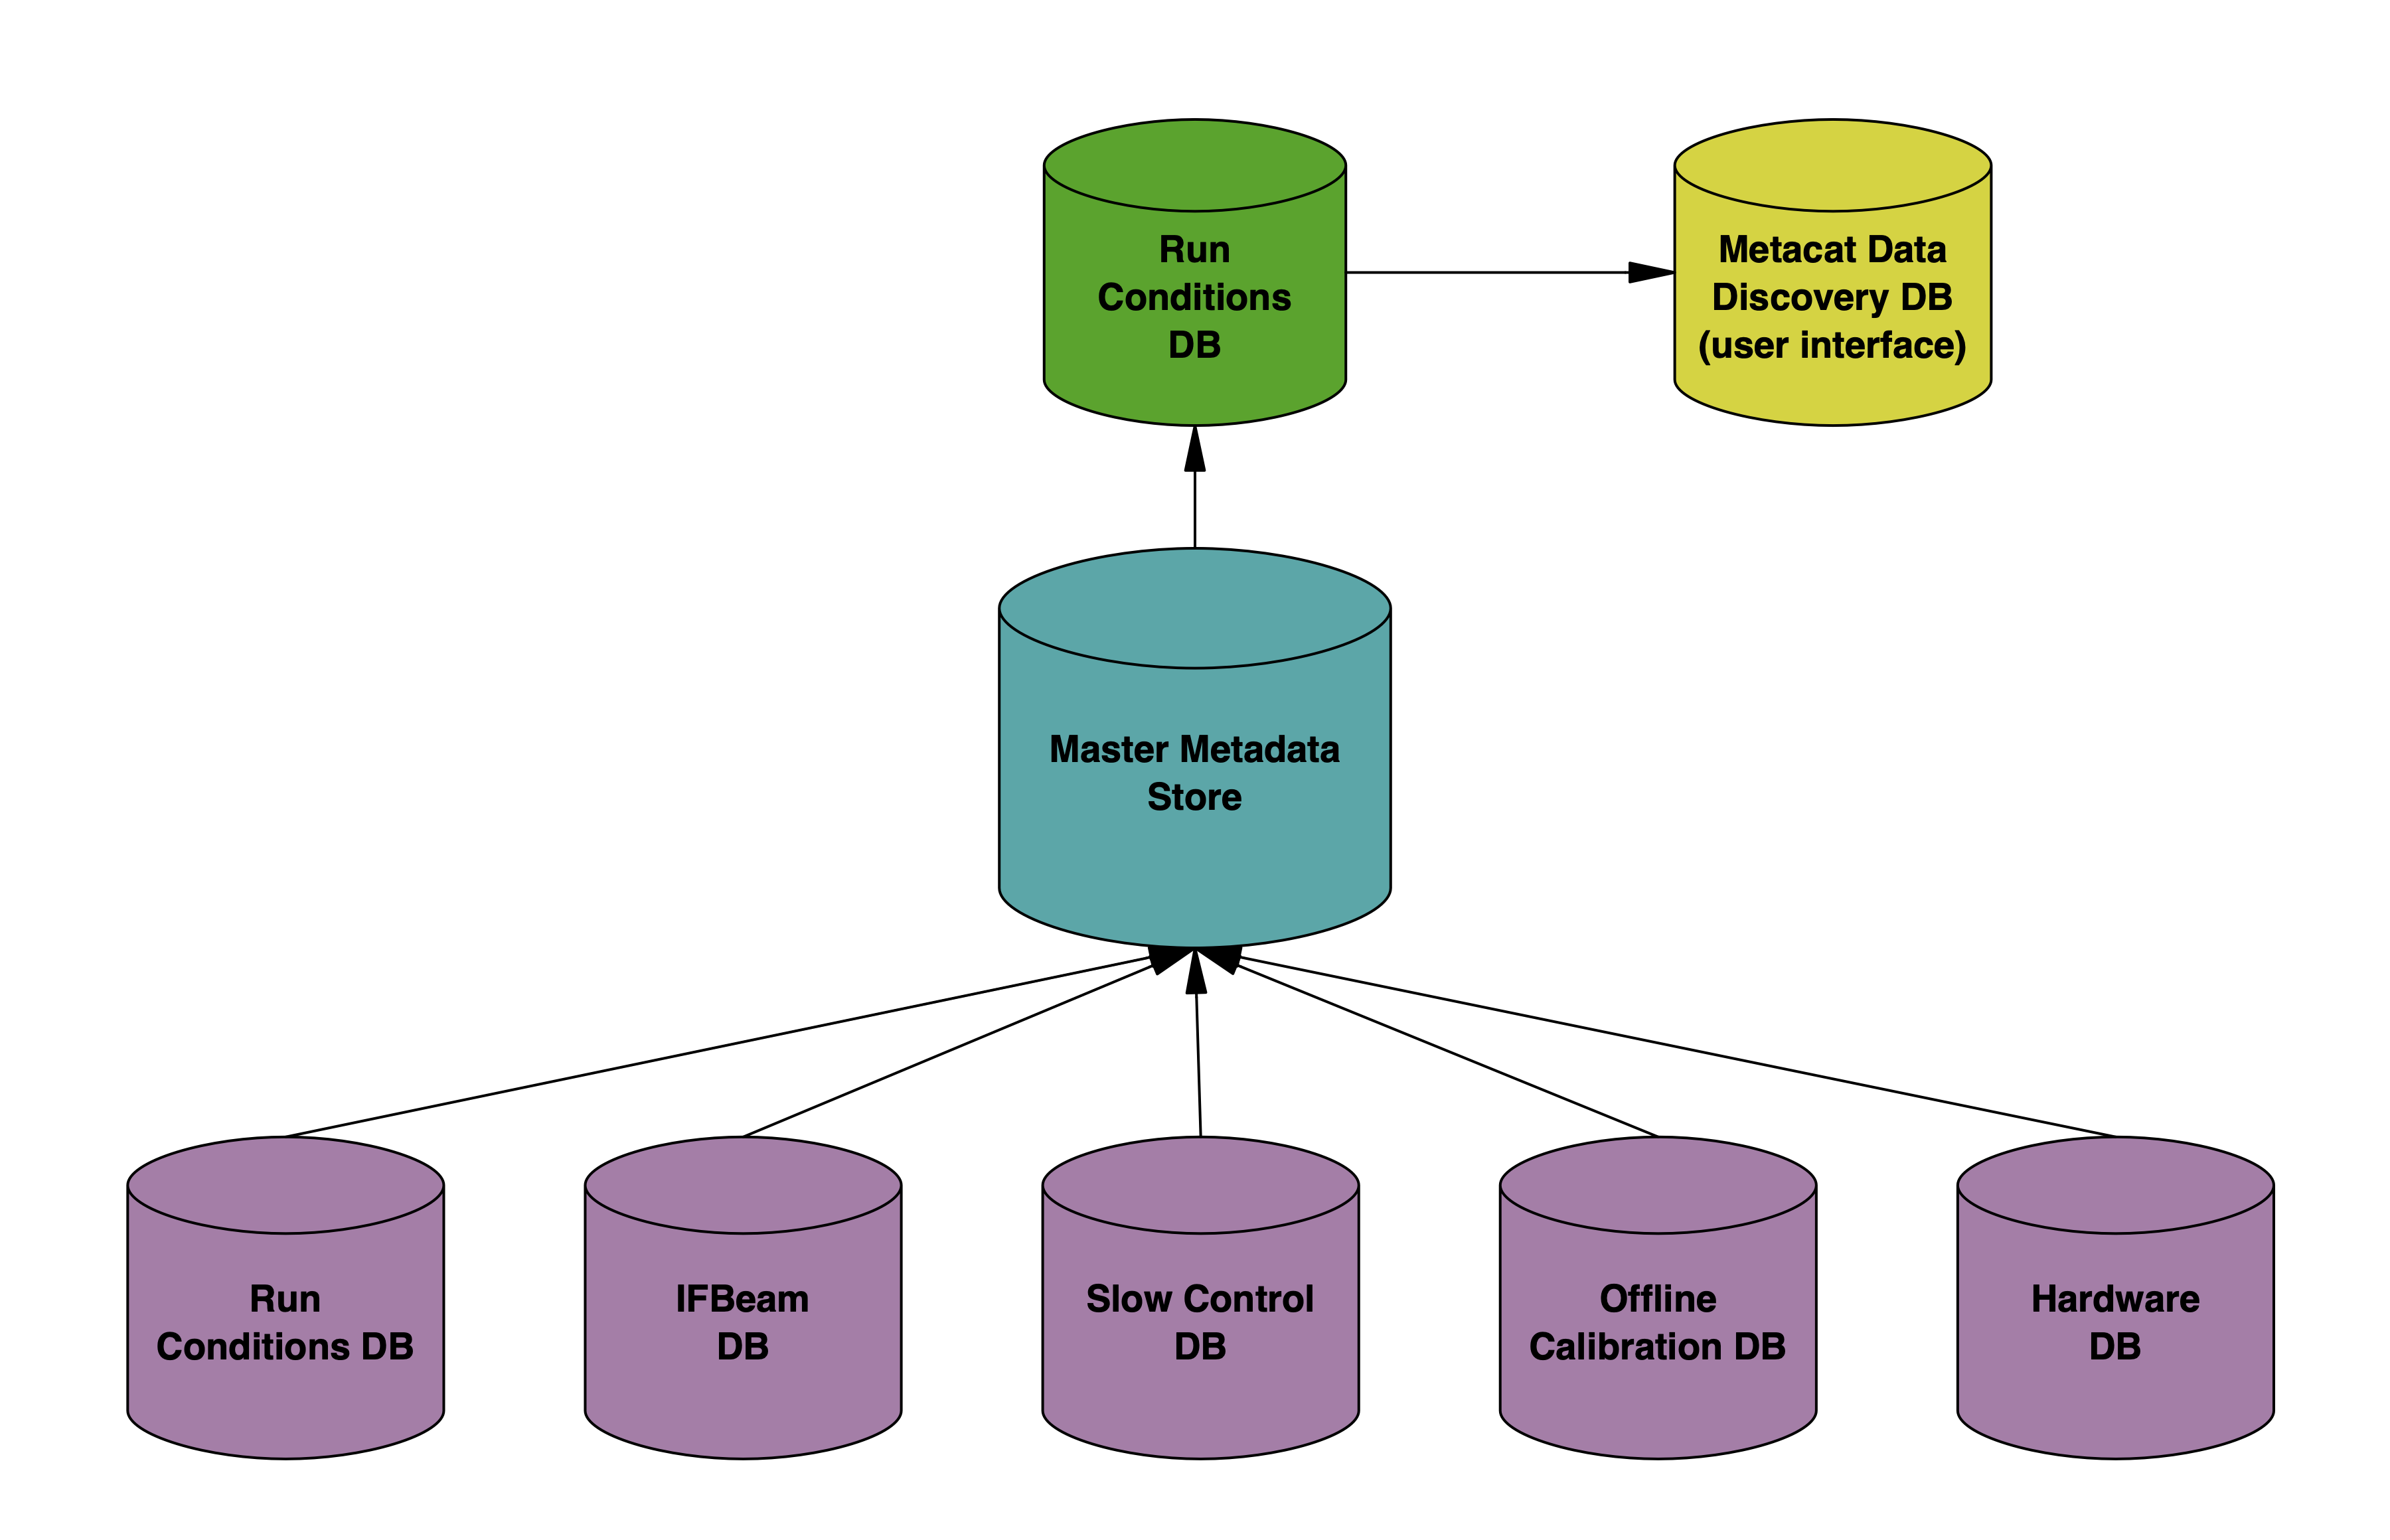
\includegraphics[width=.9\columnwidth]{graphics/Databases/DBSystem-cartoon.png}
\end{dunefigure}


The conditions database will contain interpolated (e.g., slow controls) and non-interpolated (e.g., run configurations) information. Interpolated information may more naturally be keyed by time-stamps, while configurations are more naturally keyed by run number. Tools will need to be developed to handle these two %anne cases 
types of database content. 

In order to provide a balance between the availability of the largest set of metadata possible  and allowing schema evolution,  the conditions database will employ an unstructured approach utilizing an unstructured No-SQL database \dword{ucondb}~\cite{bib:ucondb}. The \dword{ucondb} where metadata from several specific databases and sources, like the \dword{daq} system, will be stored in ``blobs'' corresponding to temporal periods (run, time blocks, or \dwords{iov2}). Each blob will contain a \dword{json}-formatted record of metadata. Folders will be used to hold metadata corresponding to time and run keys. Tools will be provided to correlate between the the two. 

An example of a metadata blob~\footnote{This metadata is taken from \dword{iceberg}, a small DUNE-related experiment. \dword{protodune}, and DUNE, conditions metadata will be significantly larger, O(10~MB).}

\begin{verbatim}
{
    "Run Number": 648,
    "Start Time": " 2019-03-04T22:23:40",
    "End Time": " 2019-03-04T22:25:31",
    "Pulser Mode": 2,
    "Pulser DAC": 7,
    "Gain": 2,
    "Shaping": 2,
    "AC Coupling": 0,
    "Baseline High": 1,
    "Leak High": 1,
    "Leak 10x": 0,
    "FE Buffer": 0,
    "Events": 228,
    "Filename": " iceberg_r000648_sr01_20190304T222340_1_dl1.root",
    "isduplicate": 0,
    "DAQ Config": "iceberg_g2s2b1_maskWIB001FEMB4_pulser7_00001"
}
\end{verbatim}

A smaller relational database will contain a subset of the metadata most often queried by users. This will enable much faster queries than accessing the unstructured conditions database directly.

\subsection{Conditions Database for DUNE}

An unstructured conditional database was used for the \dword{protodune} experiment. Collections of metadata corresponding to \dword{protodune} runs were stored as text-based ``blobs'' in key-value pairs. For the first \dword{protodune} run the blobs contained \dword{fhicl}-formatted information and Run II blobs will be in \dword{json} format. The \dword{ucondb} format enables the capture of a comprehensive set of metadata without the need for a strict schema to be determined in advance of operating the database. Postgres provides the ability to utilize folders in the database structure, which can be used for versioning should the metadata coming from any source change over time. Folders can also keep metadata keyed by run number separate from that keyed by time. Tools can be used to match either up to any \dword{iov2}-based query. Further details of the use of the \dword{ucondb} for \dword{protodune} can be found in Section~\ref{sec:runconfigPD} 

\section{Run Configuration Database  \hideme{Buchanan and Laycock - draft}}
\label{sec:db:config}  

The run configuration database contains the intended configuration of the detectors during data collection -- physics or otherwise. 

Metadata contained in the run configuration database includes hardware settings, run type, and run start and end times. Table~\ref{table:runconfig} contains some examples of typical metadata that will be contained in the run configuration database. 

\begin{dunetable}[Run configuration database example]
{l  l } 
{table:runconfig}
{Example metadata values and types stored in the run configuration database.}
%\begin{table}[h!]
%\centering
% \begin{tabular}{l  l } 
% 
 Metadata Value & Type  \\ [0.5ex] 
 
Start of run   &  Time \\ \toprowrule
Readout window size  & Integer  \\ \colhline
Readout trigger type  &  Integer \\  \colhline
Readout firmware version &  Integer \\  \colhline
Baseline start &  Integer \\  \colhline
Shifter comments &  Text \\  \colhline
Run end status & Integer \\  
%
%\end{tabular}
%\caption{Example metadata values and types stored in the run configuration database.}
%\label{table:runconfig}
%\end{table}
\end{dunetable}

The majority of run configuration metadata comes from the configuration files used by the \dword{daq} system during run execution. Some additional metadata collected at the end of the run, or shortly thereafter, may also be included. Examples are run completion status and comments made by the shifter during the run or in run-related checklists.

Parameters used to configure the run will be collected and packed into \dword{json}-formatted blocks in a single blob corresponding to a \dword{daq} run.   

\subsection{Run Configuration Database for ProtoDUNE}
\label{sec:runconfigPD}

 Following the completion of a run, the run configuration parameters corresponding to the run are read from the mongoDB and packed into a single %anne"blob" 
 blob of key-value pairs in \dword{json} format. Any additional information, such as end-of-run time, are added to the blob, which is then transferred to the \dword{ucondb} at \dword{fnal}. A typical metadata blob is on order 10\,MB in and contains more information than most users will want to use. An additional step of reducing the metadata is performed to produce a subset of metadata needed by offline users. The reduced set of metadata is stored in a single table in a relational database referred to as the ``run history database.'' An interface is provided to users, enabling them to retrieve run numbers and file locations based on queries of the history database. 

For %anne Run II of 
\dword{protodune2} the conditions \dword{db} will include metadata from multiple sources, as will be the case for DUNE. Metadata from the beam conditions database (IFBeam), the slow controls database, and data quality data database (DQMD),
\todo{(anne) data quality management database?} will be included in addition to the run configuration information. The \dword{ucondb} is able to store data keyed by either non-interpolated values (run number) or interpolated values (timestamps). Users are then able to access information using run numbers or dates and times.


\begin{dunefigure}
[Flow of metadata from \dshort{protodune} DAQ to user interface]
{fig:protoconditions} 
{Flow of metadata from \dword{protodune} \dword{daq} to user interface.}
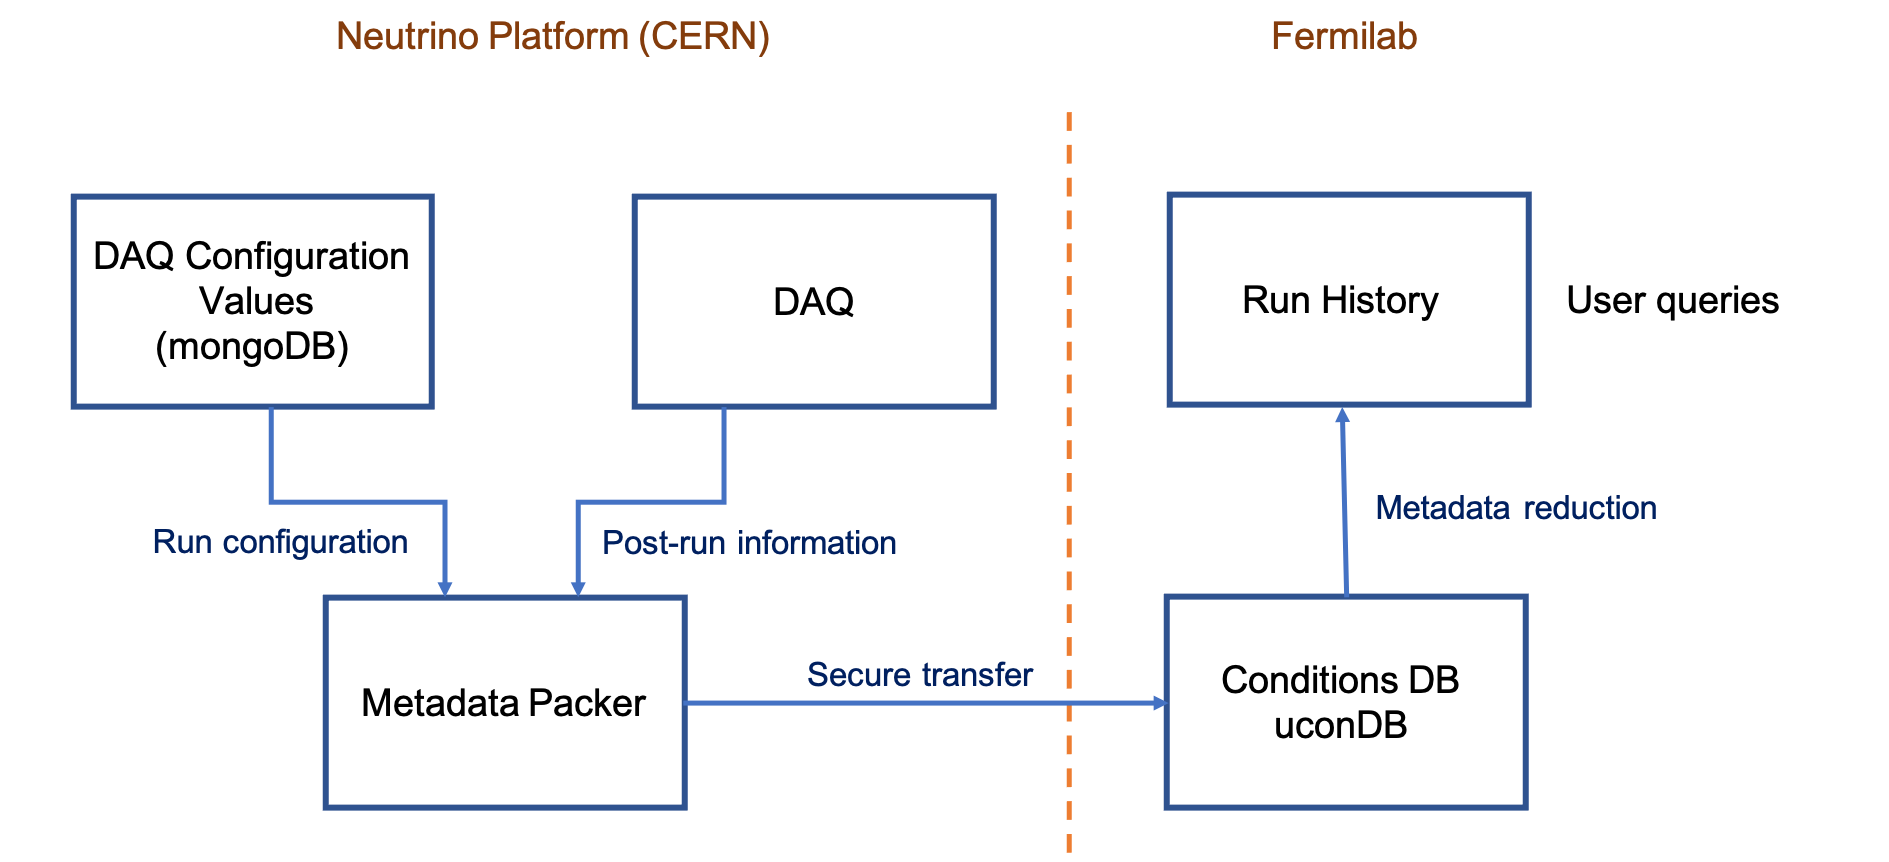
\includegraphics[width=.9\columnwidth]{graphics/Databases/Conditions_ProtoDUNE.png}
\end{dunefigure}

\section{Data Quality and Monitoring Database  \hideme{Buchanan and Laycock - draft}}
\label{sec:db:dqm}  

The \dword{dqmd} contains metadata derived from data collected during operation of the DUNE detectors. The \dword{dqmd}  is an online database and interfaces with the conditions database directly or via an offline data quality database. \todo{ (anne) \dword{dqm} db?}

\section{Offline Calibration Database  \hideme{Buchanan and Laycock - draft}}
\label{sec:db:calib} 

The calibration database contains calibration constants determined from collected data corresponding to  \dword{iov2}. The calibration metadata will result from offline calculations using data collected from the DUNE detectors.

There will generally be multiple versions of calibration constants corresponding to the same interval of validity. These versions will be contained within the database and accessible to users.  

\section{Slow Control Database \hideme{Buchanan/Laycock - draft}}
\label{sec:db:slowcontrol}  

The slow control \dword{db} contains metadata specific to the state of detector during the time data were collected as well as before and after. Examples of slow control metadata are measurements of power supply voltages and currents, and temperatures. Each slow control quantity corresponds to a particular device. The slow control \dword{db} metadata is time-indexed and hence must be interpolated, Additionally, different devices can be sampled at different rates.

The slow control metadata is captured via a Supervisory Control and Data Acquisition (\dword{scada}) system that is the responsibility of the Slow Control and Monitoring group. The \dword{scada}  system pushes values to a back-end database, where the \dword{db} flavor is tied to the \dword{scada} solution. 

The \dword{scada}  system can provide data reduction through filtering prior to insertion of metadata into the back-end \dword{db}, which reduces the workload on any API used to move the metadata to conditions database. 

\subsection{Slow Control Database for ProtoDUNE}
\label{sec:slowcontrolPD}

The \dword{protodune} experiment has been using an Oracle~\footnote{Oracle\textcopyright, \url{https://www.oracle.com}} back-end \dword{db} for the slow control system. As Fermilab Scientific \todo{(anne) did you mean Core? }Computing Division does not support Oracle, the information from the Oracle database must be extracted and moved into a Postgres \dword{db} at Fermilab. Any filtering of the metadata not handled by the \dword{scada}  system when populating the Oracle database can be handled by the API that transfers the Oracle records to Postgres.

No data filtering was provided by the \dword{scada}  for \dword{protodune} Run I but for Run II it is expected that the Oracle \dword{db} will filtered based on needs of offline users.  

\section{Beam Conditions Database - IFBeam  \hideme{Buchanan and Laycock - draft}}
\label{sec:db:ifbeam}  

The beam conditions database, \dword{ifbeam}~\cite{ifbeam} will contain metadata related to the condition extracted beam and corresponding diagnostics.  The functional form of this database is essentially the same as that of the slow control database. A large number of devices are sampled into the \dword{ifbeam} \dword{db}. The \dword{ifbeam} metadata transferred to the conditions \dword{db} will be a coarser subset of the original set.

Quantities contained in the \dword{ifbeam} \dword{db} include beam currents, horn currents and polarities, and beam monitoring instrument metadata.

\begin{dunetable}
[Example IFBeam metadata]
{l  l } 
{table:ifbeam}
{Example metadata values and types stored in the \dword{ifbeam} database.}
%\begin{table}[h!]
%\centering
% \begin{tabular}{l  l } 
% 
 Metadata Value & Type  \\ \toprowrule [0.5ex] 
% 
Horn 1 Polarity &  Integer \\ \colhline
Horn 2 Polarity  & Integer  \\ \colhline
Beam current & Float \\  
%
%\end{tabular}
%\caption{Example metadata values and types stored in the run configuration database.}
%\label{table:ifbeam}
%\end{table}
\end{dunetable}


\section{Hardware Database  \hideme{Buchanan and Laycock - draft}}
\label{sec:db:hwdb}  

The purpose of the hardware database (\dword{hwdb}) is to track the lineage of hardware components. In this context a component can be a sub-detector module or any of the individual parts comprising it. For example, a readout board is a component as is a mezzanine daughter board or programmable logic chip mounted on the readout board. The lowest level component tracked within the \dword{hwdb} will be unique to the corresponding hardware system. 

A requirement of the \dword{hwdb} is that any component, or part, stored in the database must have a unique identification number assigned to it. A separate database, under the responsibility of the DUNE Integration group, 
\todo{(anne) is this a formal group, and is this the title?} will be the source of the unique part ID numbers assigned to each component. The part numbers will be designated as shown in Table~\ref{table:partsid}. The project field corresponds to DUNE detectors (D), integration (I), LBNF (L), and future project (P). The project identifier is allocated by the project management team while the other identifiers are left for the various hardware consortia to assign. There are additional fields not listed as they are not relevant to the \dword{hwdb}.  More details of the parts identification number can be founds in~\cite{bib:cernedms2505353}.

\begin{dunetable}
[Hardware database component IDs]
{l l l l l l} 
{table:partsid}
{Unique parts identification number assigned to each component stored in the hardware database.}
Project & System ID & Subsystem ID & Item Type ID & Dash & Item Number  \\ \toprowrule 
D/I/L/P & 01-99 & 001-999 & 0001-FFFF & - & 0001-FFFF \\  
\end{dunetable}

Hardware \dword{db} metadata will reflect the complete lifetime of the detector component, including the following:

\begin{itemize}
\item Procurement, 
\item Fabrication,
\item Quality control testing,
\item Shipping and storage,
\item Installation, and
\item Maintenance. 
\end{itemize}

The relationships between components will be reflected in the \dword{hwdb}. Metadata corresponding to multiple instances of events such as \dword{qc} tests will be handled using time series within the database. 

The database group will provide an interface to the \dword{hwdb} and each hardware consortium will be required to ensure that their metadata is inserted into the database. Given the wide range of hardware groups and the international nature of the experiment it is expected that the various consortia will develop different metadata capture and temporary storage solutions. The database group will consult with the consortia but ultimately the consortia will need to provide their own APIs for record insertion into the \dword{hwdb}.  


\section{Service and Maintenance  \hideme{Buchanan and Laycock - draft}}
\label{sec:db:service}  

Most, if not all, of the DUNE databases will operate in advance of the full DUNE experiment coming online and these databases will need to be maintained and serviced once they are operational. 

The second run of the \dword{protodune} experiment (\dword{protodune2}) will employ a suite of databases that will be the precursors to the full database system that will be in place for DUNE. Each of these databases (run configuration, beam instrumentation, conditions, slow controls, and hardware) will require stable monitoring, maintenance, and service to address operational issues that will arise in the lead up to and during %anne the running of the \dword{protodune} II experiment. 
\dword{protodune2} operations.

Monitoring will be achieved using automated web-based tools \todo{[ref needed]|} and responses to offline database issues will be made within an 8-hour period corresponding to a typical operation or production ``shift.'' For \dword{protodune2} databases will be located at both \dword{fnal} and \dword{cern}, both of which have a long history of database support.

\section{Development Plans  \hideme{Buchanan and Laycock - draft}}

There are a number of database-related projects where R\&D is needed or underway. 

\subsection{Slow Control Database}

The \dword{scada}  system chosen for Run I and II of the \dword{protodune} experiment was WinCC with Oracle as the back-end \dword{db}. This system is well tested and it is relatively trivial to transfer information from the Oracle \dword{db} to a \dword{postgres} \dword{db} located at Fermilab. Given the fact that Oracle-based \dwords{db} are not guaranteed to be supported for the life of DUNE it would be beneficial to use a solution that enables a \dword{postgres} back-end.  We are investigating potential solutions. 

\subsection{Database Access for High-Performance Computing Facilities}

As DUNE will utilize \dword{hpc}   facilities for some analysis tasks it is important that \dword{db} access is manageable when tens, or hundreds, of thousands of processes are distributed across an \dword{hpc}   cluster. Studies on how scaling on such systems can be handled without overwhelming the conditions \dword{db} with an enormous number of simultaneous queries are required. %anne need to be undertaken. 

\subsection{Person Power Estimates}

The personnel needs will be largely front-loaded as the database systems are researched, implemented, and tested. The databases requiring the most effort will be the slow control, run configuration, calibration, and conditions databases.  

Estimates of the personnel needs over the next three years are given in Table~\ref{table:dbneeds}. 


\begin{dunetable}
[Person-power estimates for database development]
{l l l l l}
{table:dbneeds}
{Database group person-power needs over next three years.}
% \begin{table}[h!]
% \centering
%  \begin{tabular}{l l l l l} 
 
 Database & FY21 & FY22 & FY23 & Total \\ \toprowrule
 
Conditions \dword{db} &  0.7 FTE & 0.5 FTE & 0.5 FTE & 1.7 FTE$\cdot$yr \\ \colhline
Slow control \dword{db} &  0.5 FTE & 0.3 FTE & 0.3 FTE & 1.1 FTE$\cdot$yr \\ \colhline
Run Configuration \dword{db} &  0.5 FTE & 0.3 FTE & 0.3 FTE & 1.1 FTE$\cdot$yr \\ 
%%\end{tabular}
%\caption{Database group person power needs over next 3 years.}
%\label{table:dbneeds}
%\end{table}
\end{dunetable}
\end{document}